\documentclass[11pt,a4paper,twocolumn]{article}
\usepackage[portuguese]{babel}
\usepackage[colorlinks,allcolors=blue]{hyperref}
\usepackage[margin=1in]{geometry}
\usepackage[utf8]{inputenc}
\usepackage{amsmath}
\usepackage{graphicx}
\newcommand{\dpar}[1]{\left(#1\right)}
\newcommand{\un}[1]{\mathrm{#1}}

\DeclareMathOperator{\sen}{sen}
\DeclareMathOperator{\pr}{pr}

\title{Física Geral I: Lista de exercícios 4}

\author{Data de entrega: 6 de junho de 2018}

\date{}

\begin{document}
\maketitle
\begin{enumerate}
\item Um bloco de $5\,\un{kg}$ se encontra sobre uma mesa como
  mostrado na figura~\ref{fig:1}. (i)~Determine o módulo e a direção
  da força normal sobre o bloco. (ii) Se a superfície da mesa é
  rugosa, determine o módulo e a direção da força de atrito sobre o
  bloco para que ele se mova com velocidade constante. (iii) Se a
  superfície da mesa é lisa, determine o módulo e a direção da
  aceleração do bloco.
  \begin{figure}[h]
    \centering
    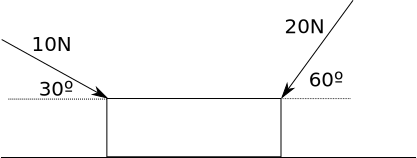
\includegraphics[width=0.45\textwidth,keepaspectratio]{lista4-questao1.pdf}
    \caption{Questão 1.}
    \label{fig:1}
  \end{figure}
\item A figura~\ref{fig:2} ilustra dois blocos sobre uma mesa. As
  massas dos blocos $A$ e $B$ são $2\,\un{kg}$ e $5\,\un{kg}$
  respectivamente. O coeficiente de atrito da superfície da mesa é
  $0{,}1$ (módulo da força de atrito é igual ao módulo da força normal
  vezes o coeficiente de atrito). Se não há força de atrito entre os
  blocos, determine a aceleração dos blocos.
  \begin{figure}[h]
    \centering
    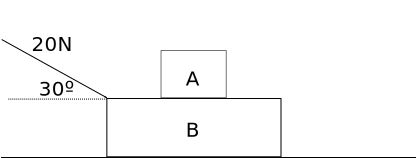
\includegraphics[width=0.45\textwidth,keepaspectratio]{lista4-questao2.pdf}
    \caption{Questão 2.}
    \label{fig:2}
  \end{figure}
\item Na figura~\ref{fig:3} as massas dos blocos $A$ e $B$ são
  $50\,\un{kg}$ e $100\,\un{kg}$ respectivamente. (i) Qual deve ser a
  força de atrito sobre o bloco $B$ para que o bloco $A$ esteja em
  repouso? (ii) Se a superfície sobre a qual o bloco $B$ se encontra é
  lisa, determine o módulo e a direção da aceleração dos blocos.
  \begin{figure}[h]
    \centering
    \includegraphics[width=0.45\textwidth,keepaspectratio]{lista4-questao3.pdf}
    \caption{Questão 3.}
    \label{fig:3}
  \end{figure}
\end{enumerate}
\end{document}